\documentclass[tikz,border=9pt]{standalone}
\usepackage{amsmath,amssymb}
\usetikzlibrary{arrows.meta,positioning,calc}
\begin{document}
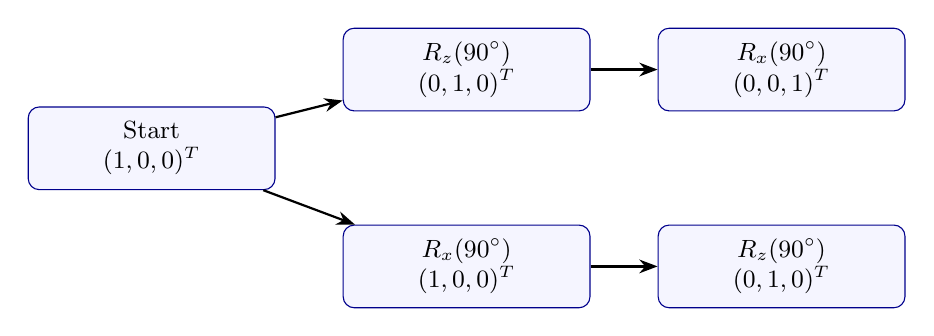
\begin{tikzpicture}[font=\small,arr/.style={-{Stealth},thick},box/.style={draw=blue!55!black,rounded corners,fill=blue!4,align=center,text width=2.9cm,minimum height=1.05cm}]

\node[box] (v) at (0,0) {Start\\$(1,0,0)^T$};
\node[box] (z) at (4,1) {$R_z(90^\circ)$\\$(0,1,0)^T$};
\node[box] (x) at (8,1) {$R_x(90^\circ)$\\$(0,0,1)^T$};
\node[box] (x2) at (4,-1.5) {$R_x(90^\circ)$\\$(1,0,0)^T$};
\node[box] (z2) at (8,-1.5) {$R_z(90^\circ)$\\$(0,1,0)^T$};
\draw[arr] (v)--(z);\draw[arr] (z)--(x);\draw[arr] (v)--(x2);\draw[arr] (x2)--(z2);

\end{tikzpicture}
\end{document}
